%
% Copyright (c) 2017 Intel Corporation
%
% Permission is hereby granted, free of charge, to any person obtaining a copy
% of this software and associated documentation files (the "Software"), to
% deal in the Software without restriction, including without limitation the
% rights to use, copy, modify, merge, publish, distribute, sublicense, and/or
% sell copies of the Software, and to permit persons to whom the Software is
% furnished to do so, subject to the following conditions:
%
% The above copyright notice and this permission notice shall be included in
% all copies or substantial portions of the Software.
%
% THE SOFTWARE IS PROVIDED "AS IS", WITHOUT WARRANTY OF ANY KIND, EXPRESS OR
% IMPLIED, INCLUDING BUT NOT LIMITED TO THE WARRANTIES OF MERCHANTABILITY,
% FITNESS FOR A PARTICULAR PURPOSE AND NONINFRINGEMENT. IN NO EVENT SHALL THE
% AUTHORS OR COPYRIGHT HOLDERS BE LIABLE FOR ANY CLAIM, DAMAGES OR OTHER
% LIABILITY, WHETHER IN AN ACTION OF CONTRACT, TORT OR OTHERWISE, ARISING
% FROM, OUT OF OR IN CONNECTION WITH THE SOFTWARE OR THE USE OR OTHER DEALINGS
% IN THE SOFTWARE.
%

\newcommand{\repoTopPath}{../../..}
\newcommand{\commonPreamblePath}{\repoTopPath/common/latex/common_preamble.tex}
\input \commonPreamblePath

%----BEGIN TYPESETTING----------------------------------------------------------
\begin{document}
\sffamily

% create our own title area rather than \begin{titlepage} or \maketitle
\begin{center}
\let\savethefootnote\thefootnote
\let\thefootnote\relax\footnote{Intel, and Quartus are trademarks of Intel Corporation or its subsidiaries in the U.S. and/or other countries.}
\addtocounter{footnote}{-1}
\let\thefootnote\savethefootnote
\hspace{-1em}
\let\savethefootnote\thefootnote
\let\thefootnote\relax\footnote{Other names and brands may be claimed as the property of others.}
\addtocounter{footnote}{-1}
\let\thefootnote\savethefootnote
\hspace{-1em}
\LARGE{Interacting with FPGA Designs using System Console}\\[1em]
\end{center}

\begin{flushleft}
\normalsize{PDF created: \today}\\
\normalsize{Validated using tools release: \TheToolsReleaseVersion}
\end{flushleft}

% make an entry in the PDF bookmarks for the TOC
\pdfbookmark[0]{Contents}{sumario_label}
% insert the default TOC format
\tableofcontents

%----NEW SECTION DEFINITION-----------------------------------------------------
\section*{Overview}
% must manually add TOC reference for unnumbered section
\addcontentsline{toc}{section}{Overview}
%----NEW SECTION DEFINITION-----------------------------------------------------

\begin{flushleft}
\noindent
This tutorial demonstrates how to use the System Console debugging tool to program a compiled FPGA design into an FPGA device, then access the hardware modules instantiated in that FPGA design.  This System Console tutorial is based on the FPGA design created in the \textquote{My First Qsys System} tutorial.  In that tutorial you create this Qsys system:

\begin{figure}[H]
\centering
% screen shots report a density of 37.8 PixelsPerCentimeter when actual resolution
% is more like 56 PixelsPerCentimeter, so the scaling factor for 1:1 is 0.675
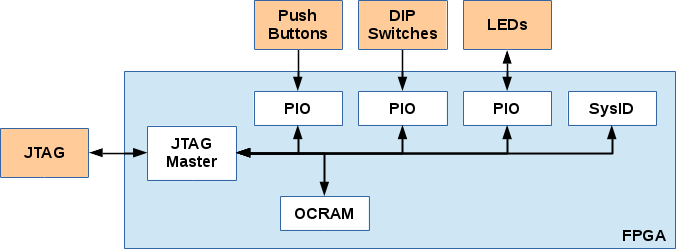
\includegraphics[scale=0.675]{qsys_block_diagram}
\caption{Qsys System Block Diagram}
\label{fig:qsys_block_diagram}
\end{figure}

In this tutorial we will demonstrate how you can interact with the Qsys system through a JTAG cable connected to the FPGA that can send read and write transactions through the JTAG master in the Qsys system to interact with the slave peripherals it is connected to.

\end{flushleft}

%----NEW SECTION DEFINITION-----------------------------------------------------
\section*{Prerequisites}
% must manually add TOC reference for unnumbered section
\addcontentsline{toc}{section}{Prerequisites}
%----NEW SECTION DEFINITION-----------------------------------------------------

\begin{flushleft}
\noindent
The following are required:

\begin{itemize}

\item Windows\textsuperscript{*} or Linux\textsuperscript{*} development host PC

\item Installed Intel\textsuperscript{\textregistered} Quartus\textsuperscript{\textregistered} Prime Software Suite.  Either the Lite or Standard Edition, but not the Pro Edition.

\item Completed Intel Quartus software project from \textquote{My First Qsys System}

\begin{itemize}

\item Either follow the tutorial steps presented \href{\TheReleasesURL/writeup_MyFirstQsysSystem.pdf}{\underline{here}}.

%\item Or, you can extract this PDF attachment to your local file system: \textattachfile[
%	color=0.0 0.678 0.937,
%	mimetype=application/zip,
%	description={ZIP Archvie File: blink.zip}
%]{../blink_archive/blink.zip}{\textbf{blink.zip}}. Right click on the PDF attachment link and your PDF reader should present a pop-up menu with an option to save the attachment to your local file system.
\item Or, you can download an archive of the required contents from that tutorial to your local file system \href{\TheReleasesURL/blink_for_InteractSystemConsole.zip}{\underline{here}}.

\end{itemize}

\item Terasic DE10-Nano board

\item Power supply for Terasic DE10-Nano

\item Mini USB cable to connect Terasic DE10-Nano USB Blaster II port with PC

\end{itemize}

\end{flushleft}

%----NEW SECTION DEFINITION-----------------------------------------------------
\section*{Preparing the Terasic DE10-Nano Board}
% must manually add TOC reference for unnumbered section
\addcontentsline{toc}{section}{Preparing the DE10-Nano Board}
%----NEW SECTION DEFINITION-----------------------------------------------------

\begin{flushleft}
\noindent

This section describes how to prepare the Terasic DE10-Nano board for use in this tutorial.

\begin{enumerate}[
	label=\textbf{Step \arabic*.},
	leftmargin=*,
	widest={00},
	align=left]

\item Remove the microSD\textsuperscript{*} card from your Terasci DE10-Nano board and store it in a safe place.  During this tutorial you will not need the microSD card at all.

\item Plug the mini USB cable into the USB-Blaster II connector of the Terasic DE10-Nano board.  Then plug the other end of the USB cable to your host PC.

\begin{figure}[H]
\centering
% screen shots report a density of 37.8 PixelsPerCentimeter when actual resolution
% is more like 56 PixelsPerCentimeter, so the scaling factor for 1:1 is 0.675
\scriptsize{Image used with permission from Terasic Technologies Inc.}
\newline
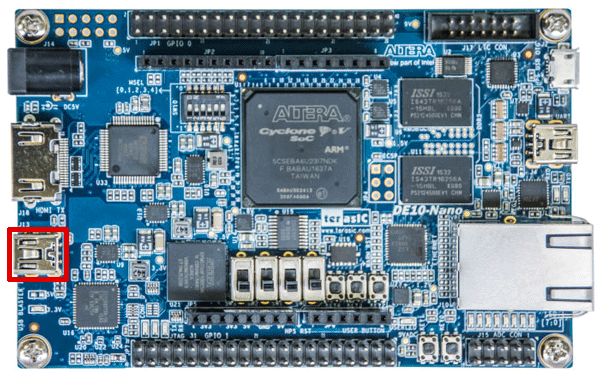
\includegraphics[scale=0.675]{de10-nano_jtag}
\caption{USB-Blaster II Connector on Terasic DE10-Nano Board}
\label{fig:de10-nano_jtag}
\end{figure}

\newpage

\item Power the Terasic DE10-Nano board by inserting the power supply cord into the power connector on the Terasic DE10-Nano board.

\begin{figure}[H]
\centering
% screen shots report a density of 37.8 PixelsPerCentimeter when actual resolution
% is more like 56 PixelsPerCentimeter, so the scaling factor for 1:1 is 0.675
\scriptsize{Image used with permission from Terasic Technologies Inc.}
\newline
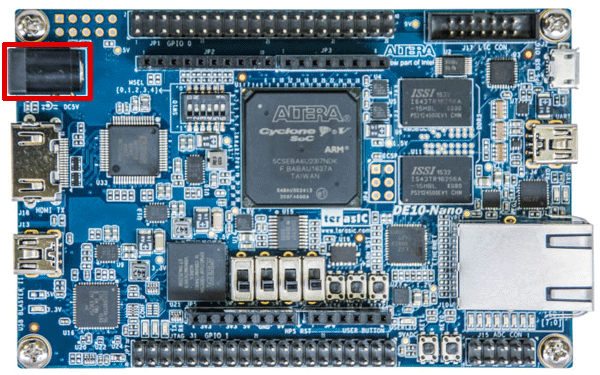
\includegraphics[scale=0.675]{de10-nano_pwr}
\caption{Power Connector on Terasic DE10-Nano Board}
\label{fig:de10-nano_pwr}
\end{figure}

\end{enumerate}

\end{flushleft}

\newpage

%----NEW SECTION DEFINITION-----------------------------------------------------
\section*{Getting Started with System Console}
% must manually add TOC reference for unnumbered section
\addcontentsline{toc}{section}{Getting Started with System Console}
%----NEW SECTION DEFINITION-----------------------------------------------------

\begin{flushleft}
\noindent

This section describes how to use System Console to download the FPGA design into the FPGA device, and then interact with the JTAG master inside the Qsys system to read and write the slave peripherals that it is attached to.  It also demonstrates JTAG link debug and Qsys system health observability provided by System Console.

\begin{enumerate}[
	label=\textbf{Step \arabic*.},
	leftmargin=*,
	widest={00},
	align=left]

\item With the \textbf{blink} project from the previous tutorial open in the Intel Quartus software tool, start by launching System Console from the \texttt{Tools->System Debugging Tools->System Console} menu.

\begin{figure}[H]
\centering
% screen shots report a density of 37.8 PixelsPerCentimeter when actual resolution
% is more like 56 PixelsPerCentimeter, so the scaling factor for 1:1 is 0.675
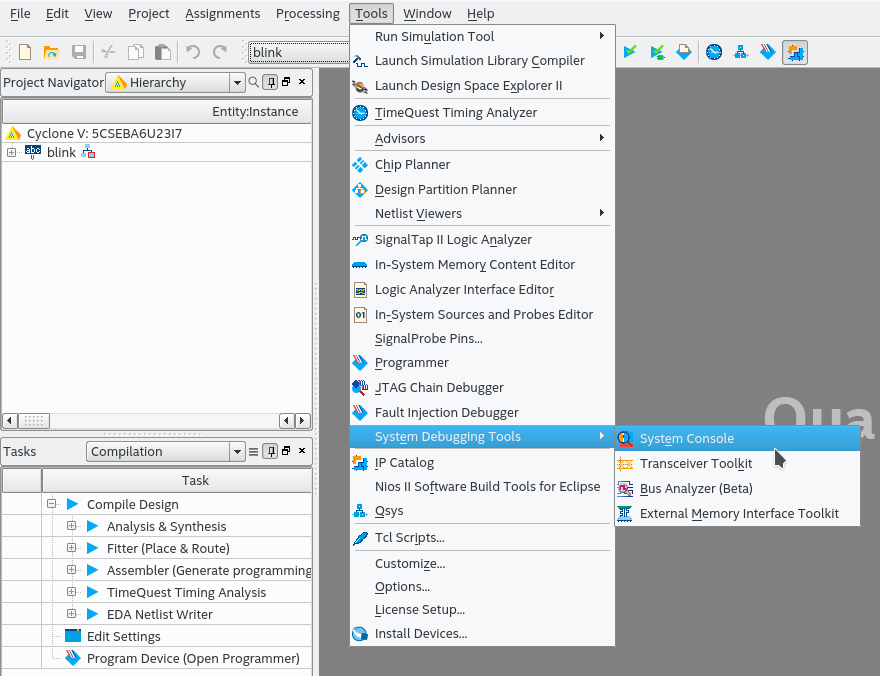
\includegraphics[scale=0.675]{01-system-console-menu}
\caption{System Console Menu}
\label{fig:01-system-console-menu}
\end{figure}

\newpage

\item The System Console tool launches and looks for available devices on available JTAG cables.  To list the available devices, type the command \textbf{get\_service\_paths device} at the \textbf{\%} prompt in the \textbf{TCL Console} pane in the bottom right corner of the System Console window.

\begin{tcolorbox}[
	colback=MyMintedBGColor,
	colframe=MyMintedBGColor,
	]

\textbf{Note:} you can double click on the title bar of the \textbf{TCL Console} pane to expand it to the full window size.  Double click it again to reduce the pane to the original size.

\end{tcolorbox}

\begin{figure}[H]
\centering
% screen shots report a density of 37.8 PixelsPerCentimeter when actual resolution
% is more like 56 PixelsPerCentimeter, so the scaling factor for 1:1 is 0.675
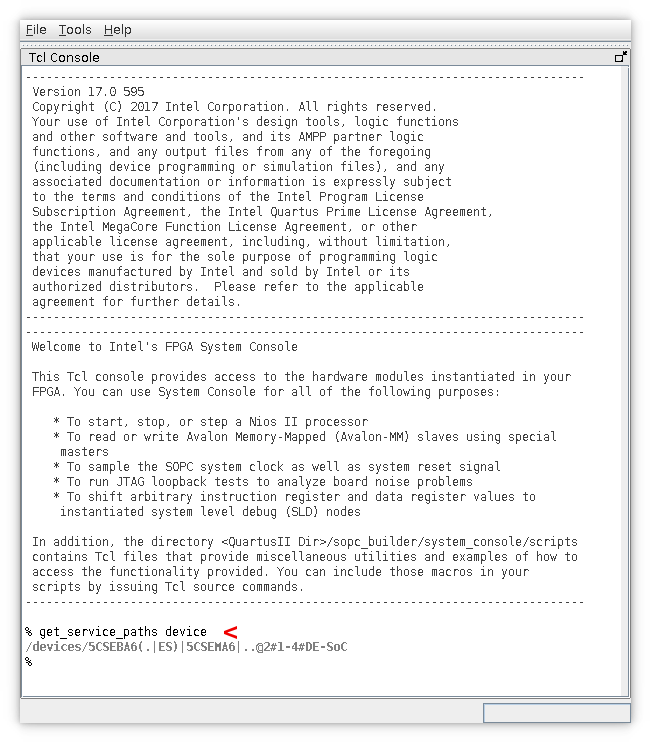
\includegraphics[scale=0.675]{02-system-console}
\caption{System Console's TCL Console}
\label{fig:02-system-console}
\end{figure}

\newpage

You can also use tab completion to complete commands as you type them and even show you what possible commands can complete from the prefix you type.  For instance if we type \textbf{get} on the command line and then press \textbf{TAB}, we see a pop-up list of all commands that begin with \textbf{get}, and we can use the up and down arrows on the keyboard to scroll the list up and down to select one of the commands.  Press \textbf{Enter} to select a command from the pop-up menu.

\begin{figure}[H]
\begin{subfigure}{0.495\textwidth}
\centering
% screen shots report a density of 37.8 PixelsPerCentimeter when actual resolution
% is more like 56 PixelsPerCentimeter, so the scaling factor for 1:1 is 0.675
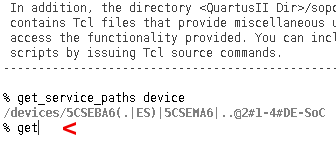
\includegraphics[scale=0.675]{02a-pre-tab}
\caption{Pre-tab Command Line}
\label{fig:02a-pre-tab}
\end{subfigure}
\begin{subfigure}{0.495\textwidth}
\centering
% screen shots report a density of 37.8 PixelsPerCentimeter when actual resolution
% is more like 56 PixelsPerCentimeter, so the scaling factor for 1:1 is 0.675
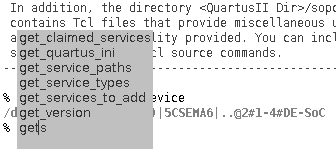
\includegraphics[scale=0.675]{02b-post-tab}
\caption{Post-tab Popup Completion Menu}
\label{fig:02b-post-tab}
\end{subfigure}
\caption{Tab Completion Example}
\label{fig:tab-completion}
\end{figure}

The TCL console history buffer can also be scrolled backward and forward using the up and down arrows on the keyboard, so you can easily recall previously executed command lines.
\newline
\newline
All of the commands generally provide help if you pass them into the \textbf{help} command, like this:

\begin{minted}[
	bgcolor=MyMintedBGColor,
	escapeinside=++
]{text}

+\%+ help get_service_paths
Returns a list of paths to nodes that implement the requested service type.
Service paths can be filtered based on a number of different optional
parameters.
	Arguments:
	  ?-type <component-type>?
	  ?-hpath <hpath-prefix>?
	  ?-device <device-path>?
	  <service-type>

Examples:
To list all paths to nodes that implement a supported service type:
	  get_service_paths <service-type>
To list all paths to nodes that implement the requested service type under a
specific hpath:
	  get_service_paths -hpath <hpath-prefix> <service-type>
To list all paths to nodes attached to a specific component type that implement
the requested service:
	  get_service_paths -type <component-type> <service-type>
To list all paths to nodes on a specific device that implement the requested
service type:
	  get_service_paths -device <device-path> <service-type>

\end{minted}

\item Program the FPGA device with the compiled design using the following commands:

\begin{minted}[
	bgcolor=MyMintedBGColor,
	escapeinside=++
]{text}

# get the service path to the device, assume there is only one device attached
+\%+ set d_path [get_service_paths device]
/devices/5CSEBA6(.|ES)|5CSEMA6|..@2#1-4#DE-SoC

# program the device with the SOF file
+\%+ device_download_sof +\$+d_path output_files/blink.sof

\end{minted}

You should see the amber \textbf{conf\_done} LED illuminate once the commands above complete.

\newpage

\item Exercise the JTAG DEBUG service path provided by the JTAG master component.

\begin{enumerate}[
	label=\textbf{Step \arabic{enumi}\alph*.},
	leftmargin=*,
	align=left]

\item Locate the JTAG DEBUG service path of the JTAG master.

\begin{minted}[
	bgcolor=MyMintedBGColor,
	escapeinside=++
]{text}

+\%+ set jb_path [get_service_paths jtag_debug]
/devices/5CSEBA6(.|ES)|5CSEMA6|..@2#1-4#DE-SoC/(link)/JTAG/
alt_sld_fab_sldfabric.node_0/phy_0

\end{minted}

\item Exercise the JTAG interface with the loop back mechanism.  This checks the physical interface on the board and into the JTAG TAP controller pins of the FPGA device.

\begin{minted}[
	bgcolor=MyMintedBGColor,
	escapeinside=++
]{text}

+\%+ jtag_debug_loop +\$+jb_path [list 1 2 4 8 15 16]
0x01 0x02 0x04 0x08 0x0f 0x10

\end{minted}

\item Sense the clock connected to the JTAG master component in the Qsys system.  This senses the clock provided to this JTAG master component inside the Qsys system.

\begin{minted}[
	bgcolor=MyMintedBGColor,
	escapeinside=++
]{text}

+\%+ jtag_debug_sense_clock +\$+jb_path
1

\end{minted}

\item Sample the clock connected to the JTAG master component.  Repeatedly sample the clock until you catch it in both the high and low state.  Again this is clock provided inside the Qsys system.

\begin{minted}[
	bgcolor=MyMintedBGColor,
	escapeinside=++
]{text}

+\%+ jtag_debug_sample_clock +\$+jb_path
0
+\%+ jtag_debug_sample_clock +\$+jb_path
0
+\%+ jtag_debug_sample_clock +\$+jb_path
1
+\%+ jtag_debug_sample_clock +\$+jb_path
1
+\%+ jtag_debug_sample_clock +\$+jb_path
0

\end{minted}

\item Sample the reset connected to the JTAG master component inside the Qsys system.  The KEY0 push button on the DE10-Nano is connected to the Qsys system reset input.  Sample the reset, press and hold the KEY0 push button and resample the reset, then release the KEY0 push button and resample the reset.

\begin{minted}[
	bgcolor=MyMintedBGColor,
	escapeinside=++
]{text}

# first sample with KEY0 not pressed
+\%+ jtag_debug_sample_reset +\$+jb_path
1
# second sample with KEY0 pressed
+\%+ jtag_debug_sample_reset +\$+jb_path
0
# third sample with KEY0 not pressed
+\%+ jtag_debug_sample_reset +\$+jb_path
1

\end{minted}

\end{enumerate}

\item Next we will exercise the master service path provided by the JTAG master.  This will require us to recall the address map produced in the previous \textquote{MyFirstQsys} tutorial.  Remember that we used the \textbf{sopc-\allowbreak create-\allowbreak header-\allowbreak files} in that tutorial to create the \textbf{master\_0.h} header file, and then we dumped all of the base address macros from that file.  To refresh your memory, here is what those addresses are:

\begin{minted}[
	bgcolor=MyMintedBGColor,
	escapeinside=++
]{c}

#define OCRAM_64K_BASE 0x0
#define LED_PIO_BASE 0x10000
#define BUTTON_PIO_BASE 0x10010
#define SWITCH_PIO_BASE 0x10020
#define SYSTEM_ID_BASE 0x10030

\end{minted}

We will set a number of TCL variables to allow us to more easily recall these base addresses in the rest of this tutorial.  Execute these commands to setup these variables:

\begin{minted}[
	bgcolor=MyMintedBGColor,
	escapeinside=++
]{text}

+\%+ set ocram 0x0
0x0
+\%+ set led 0x10000
0x10000
+\%+ set button 0x10010
0x10010
+\%+ set switch 0x10020
0x10020
+\%+ set sysid 0x10030
0x10030

\end{minted}

\begin{enumerate}[
	label=\textbf{Step \arabic{enumi}\alph*.},
	leftmargin=*,
	align=left]

\item Open the master service path.

\begin{minted}[
	bgcolor=MyMintedBGColor,
	escapeinside=++
]{text}

# locate the service path for the JTAG master component
+\%+ set m_path [get_service_paths master]
/devices/5CSEBA6(.|ES)|5CSEMA6|..@2#1-4#DE-SoC/(link)/JTAG/
alt_sld_fab_sldfabric.node_0/phy_0/master_0.master

# claim that service path so we can interact with it
+\%+ set c_path [claim_service master +\$+m_path ""]
/channels/local/(lib)/master_1

\end{minted}

\item Interact with the onchip RAM component.

\begin{minted}[
	bgcolor=MyMintedBGColor,
	escapeinside=++
]{text}

# read the onchip RAM
+\%+ master_read_32 +\$+c_path +\$+ocram 1
0x00000000

# write a pattern to the onchip RAM
+\%+ master_write_32 +\$+c_path +\$+ocram 0x1234de10

# verify the pattern remains in the onchip RAM
+\%+ master_read_32 +\$+c_path +\$+ocram 1
0x1234de10

\end{minted}

\item Interact with the LED PIO component.

\begin{minted}[
	bgcolor=MyMintedBGColor,
	escapeinside=||
]{text}

# turn on half the LEDs
|\%| master_write_32 |\$|c_path |\$|led 0x55

# turn off those LEDs and turn on the other half of the LEDs
|\%| master_write_32 |\$|c_path |\$|led 0xaa

# write a loop to toggle LED0 and LED1 every half second for 10 times
|\%| set COUNT 0
|\%| while {|\$|COUNT < 10} {
master_write_32 |\$|c_path |\$|led 0x01
after 500
master_write_32 |\$|c_path |\$|led 0x02
after 500
set COUNT [expr |\$|COUNT + 1]
}

# turn on all of the LEDs
|\%| master_write_32 |\$|c_path |\$|led 0xff

\end{minted}

\item Exercise the JTAG DEBUG service reset functionality.  Now that we have some LEDs illuminated, let's look at one more JTAG DEBUG service provided by the JTAG master component.  We have the ability to assert the reset provided into the Qsys system by the JTAG master component. To do that we use the following command:

\begin{minted}[
	bgcolor=MyMintedBGColor,
	escapeinside=++
]{text}

+\%+ jtag_debug_reset_system +\$+jb_path

\end{minted}

After executing that command, the LEDs should all turn off, returned to their reset state.  You can trigger the same reset effect by pressing the KEY0 push button like we did before.  Turn on some LEDs again and try pressing KEY0 to prove that as well.

\item Interact with the button PIO component.  The KEY1 push button is connected to this PIO peripheral.

\begin{minted}[
	bgcolor=MyMintedBGColor,
	escapeinside=++
]{text}

# read the button with KEY1 not pressed
+\%+ master_read_32 +\$+c_path +\$+button 1
0x00000001

# read the button with KEY1 pressed
+\%+ master_read_32 +\$+c_path +\$+button 1
0x00000000

# read the button with KEY1 not pressed
+\%+ master_read_32 +\$+c_path +\$+button 1
0x00000001

\end{minted}

\item Interact with the switch PIO component.  The four slide switches are connected to this PIO peripheral.

\begin{minted}[
	bgcolor=MyMintedBGColor,
	escapeinside=++
]{text}

# all switches in the up position
+\%+ master_read_32 +\$+c_path +\$+switch 1
0x0000000f

# far right switch moved down
+\%+ master_read_32 +\$+c_path +\$+switch 1
0x0000000e

# next switch to the left moved down
+\%+ master_read_32 +\$+c_path +\$+switch 1
0x0000000c

# next switch to the left moved down
+\%+ master_read_32 +\$+c_path +\$+switch 1
0x00000008

# last switch moved down
+\%+ master_read_32 +\$+c_path +\$+switch 1
0x00000000

\end{minted}

\item Interact with the system ID component.  This component contains two 32-bit words.  The first word is the ID value that we set to 0xde10de10 in the previous hardware portion of this tutorial, and the second word that represents the unix second time value when the Qsys system was generated.

\begin{minted}[
	bgcolor=MyMintedBGColor,
	escapeinside=++
]{text}

+\%+ master_read_32 +\$+c_path +\$+sysid 2
0xde10de10 0x592b40d8

\end{minted}

\newpage

\item Exercise the default slave peripheral.  Here we will demonstrate what happens when we read and write to unmapped address spans.

\begin{minted}[
	fontsize=\footnotesize,
	bgcolor=MyMintedBGColor,
	escapeinside=++
]{text}

# our peripherals are mapped into the address span from 0x0000_0000 thru
# 0x0001_0038 so we choose an arbitrary high address well above our peripherals
# and we read the 16 bytes of the default slave peripheral which should be
# initialized at device configuration to 0x0000_0000
+\%+ master_read_32 +\$+c_path 0x01000000 4
0x00000000 0x00000000 0x00000000 0x00000000

# now lets set those 4 words with a specific incrementing pattern
+\%+ master_write_32 +\$+c_path 0x01000000 [list 0x0badf00d 0x1badf00d 0x2badf00d 0x3badf00d]

# now validate that pattern repeats every 4 words
+\%+ master_read_32 +\$+c_path 0x01000000 8
0x0badf00d 0x1badf00d 0x2badf00d 0x3badf00d 0x0badf00d 0x1badf00d 0x2badf00d 0x3badf00d

# now lets write to a slave that has no write interface, like the system ID
# peripheral.  That write will not be decoded by any slave in the system and
# will be directed into the default slave
+\%+ master_write_32 +\$+c_path +\$+sysid 0xfacecafe

# now verify that the first word of the default slave was actually written
+\%+ master_read_32 +\$+c_path 0x01000000 4
0xfacecafe 0x1badf00d 0x2badf00d 0x3badf00d

\end{minted}

\end{enumerate}


\item Close the master service with this command:

\begin{minted}[
	bgcolor=MyMintedBGColor,
	escapeinside=++
]{text}

+\%+ close_service master +\$+c_path

\end{minted}

\end{enumerate}

That's it, you've interacted with the Qsys system using system console.  Continue on to the \textquote{My First HPS System} tutorial where we demonstrate how to instantiate and integrate the Hard Processor System (HPS) into your Qsys system.

\end{flushleft}

\end{document}

